\documentclass[a4 paper, 12pt]{report}
\usepackage{hyperref}
\usepackage{apacite}
\usepackage{amssymb,dsfont,amsthm,amsmath,makeidx,verbatim,latexsym,amsfonts,mathrsfs}
\usepackage{cancel}
\usepackage{graphicx}
\usepackage[none]{hyphenat}
\usepackage{csquotes}
\usepackage[english]{babel}
\addto{\captionsenglish}{%
	\renewcommand{\bibname}{REFERENCES}
	%\renewcommand{\tableofcontents}{Table of Contents}
}


\DeclareMathAlphabet{\mathpzc}{OT1}{pzc}{m}{it}
\newcommand*\rfrac[2]{{}^{#1}\!/_{#2}}

\hfuzz5pt
\theoremstyle{plain}
\newtheorem{theorem}{\textbf{Theorem}}[section]
\newtheorem{lemma}[theorem]{\textbf{Lemma}}
\newtheorem{proposition}[theorem]{\textbf{Proposition}}
\newtheorem{corollary}[theorem]{\textbf{Corollary}}
\newtheorem{claim}[theorem]{\textbf{Claim}}
\newtheorem{addendum}[theorem]{\textbf{Addendum}}
\newtheorem{definition}[theorem]{\textbf{Definition}}
\newtheorem{remark}[theorem]{\textbf{Remark}}
\newtheorem{example}[theorem]{\textbf{Example}}
\newtheorem{conjecture}[theorem]{\textbf{Conjecture}}
\newtheorem{notation}[theorem]{\textbf{Notation}}
\renewcommand{\baselinestretch}{1.50} % for the line spacing.
%\newcommand*\rfrac[2]{{}^{#1}\!/_{#2}}
\begin{document}
	\pagenumbering{roman} \baselineskip 29pt
\newcommand{\disp}{\displaystyle}
\thispagestyle{empty}


%\parindent 0pt
%\pagenumbering{roman}

%\begin{document}

\begin{center}
	\textbf{\large{CURRENCY DERIVATIVES UNDER A MINIMAL MARKET MODEL WITH RANDOM SCALING}}
\end{center}
\ \
\begin{center}
	
	BY
\end{center}
\ \
\begin{center}
	\textbf{\large{ABDULKAREEM, MUHAMMED ALI}}
\end{center}
\begin{center}
	\textbf{Matric Number 219250}
\end{center}
\begin{center}
	Submitted to the Department of  Mathematics
\end{center}
\begin{center}
	Faculty of Science  
\end{center}
\begin{center}
	University of Ibadan, Ibadan,  
\end{center}
\begin{center}
	Nigeria  
\end{center}
\begin{center}
	In Partial Fulfillment of the Award of Master of Science in Mathematics
\end{center}
\begin{center}
	In the Department of Mathematics Faculty of Science
\end{center}
\begin{center}
	University of Ibadan, Ibadan,  
\end{center}
\begin{center}
	Nigeria  
\end{center}

%\baselineskip 18pt
\begin{center}
	NOVEMBER, 2021.
\end{center}
\addcontentsline{toc}{chapter}{Title Page}
\newpage
\begin{center}
	\section*{CERTIFICATION} 
\end{center}
I certify that this project was carried out by  MR ABDULKAREEM, MUHAMMED ALI  with matriculation number 219250 in the department of Mathematics, University of Ibadan, Ibadan, Nigeria.\\
\begin{center}
	-----------------------------------------------\\
	(\textbf{Supervisor})\\
	\textbf{PROF. G.O.S. EKHAGUERE,}\\
	\textbf{B.Sc.(Ibadan), Ph.D. (London),}\\
	\textbf{Department of Mathematics,}\\
	\textbf{University of Ibadan, Ibadan, Nigeria.} 
\end{center}
%\addcontentsline{toc}{chapter}{Certification}
\addcontentsline{toc}{chapter}{Certification}

\newpage
\begin{center}
	\section*{DEDICATION}
\end{center}
\noindent
\par To my late parents Mr and Mrs Abdulkareem, in gratitude to your
amazing personalities and for being my greatest strength. I miss you both.

\addcontentsline{toc}{chapter}{Dedication}

\newpage
\begin{center}
	\section*{ACKNOWLEDGMENTS}
\end{center}
\par  Firstly, my gratitude goes to Almighty Allah for sparing my life through my
course of study.\\
\par I am deeply indebted to my supervisor, Emeritus Professor G O S. Ekhaguere,
without whose guidance and support this work will not have come to light. I am
thankful for the comments and advice you gave me from the inception of the
work to its completion, may God reward you abundantly sir.\\

\par It is a pleasure to acknowledge the impact of the distinguished Professors and
members of staff of the department in my Mathematical journey.\\

\par I am grateful to my aunt Alhaja Rafiah Sanni and her husband Alhaji Kunle Sanni and my siblings, Nada, Abdulhaqq, Wadud and Zeem for their constant financial
support and prayers.\\

\par I also want to express my sincere gratitude and thanks to my friends Gabriel Akanji,
Juwon Adeoti, Musharrafah Abolarin, Akeju John, Odunayo Ayegbusi, Austin Noah and the rest of my colleagues in the
Department for making my stay at the University of Ibadan worthwhile.\\

\par This acknowledgement will be incomplete if I failed to express my profound
gratitude to my beautiful fiancee Ilori Shukrah Oyefolashewa for all your
prayers, support and ceaseless help throughout the programme.\\

\par Finally, to those, and many others who have not been named, I express my
deep appreciation and will ever be thankful.
\addcontentsline{toc}{chapter}{Acknowledgement}

\newpage
\begin{center}
	\section*{ABSTRACT}
\end{center}
\noindent
% \par For the pricing and hedging of derivatives, this research provides an alternative,
% parsimonious stochastic volatility model to describe the dynamics of a currency
% market. The primary driving variables of the minimal market model are time transformed squared Bessel processes. A random scale characterizes the time
% transformation, allowing for realistic exchange rate dynamics. The costing of common European choices is investigated. It is demonstrated that the model
% generates implied volatility surfaces that are similar to those seen in real
% markets.
\par 
This project proposes an alternative, simple stochastic volatility model to describe the dynamics of a currency market for the pricing and hedging of derivatives. The time transformed squared Bessel processes are the fundamental driving variables in the minimal market model. The temporal transformation is defined by a random scale, which allows for realistic exchange rate dynamics. The price of popular European options is looked into. The model produces implied volatility surfaces that are similar to those seen in real markets, as shown.

\addcontentsline{toc}{chapter}{Abstract}


\newpage 
\tableofcontents
\addcontentsline{toc}{chapter}{Table of Contents}

%\newpage
%\listoftables
%\addcontentsline{toc}{chapter}{List of Tables}

\newpage
\listoffigures
\addcontentsline{toc}{chapter}{List of Figures}
%%\listoftables
%\addcontentsline{toc}{chapter}{List of Tables}


\newpage
\pagenumbering{arabic}
\numberwithin{theorem}{section}

%\chapter{GENERAL INTRODUCTION}


\chapter{GENERAL INTRODUCTION}
\section{Backgroung of Study}
\subsection{Introduction}
\noindent
\par Warren Buffett memorably described derivatives as ``financial weapons of mass
destruction''. The much vaunted - and maligned - financial products have become a dirty
word in the popular press. But without them, financial markets and the world as we
know it simply wouldn't work. Derivatives were first instruments developed to secure the
supply of commodities and facilitate trade as well as to insure farmers against crop
failures. Over time, derivatives started to serve in addition other purposes such as a
source of funding but also the search for quick profits. From history it shows that
derivatives were regulated from the very beginning.\\
The degree of regulation of derivatives varied over the years, among jurisdictions and
depended on, for example, the political but also religious contexts. Some forms of
derivatives were banned and later allowed or the other way round. The history of
derivatives also provides evidence that the first derivatives markets were ``over-the-
counter'' (OTC). However, negotiating and contracting mostly took place at specific
locations, which, early in the history of derivatives, already displayed various
characteristics of organised derivatives markets. Derivatives exchanges came later, but
once established, trading of derivatives mainly occurred on their premises. The trend
only reversed in the early 1990s.
\subsection{The Origin of Derivatives}
\noindent
\par ``If any one owes a debt for a loan, and a storm prostrates the grain, or the harvest
fail, or the grain does not grow for lack of water; in that year he need not give his creditor
any grain, he washes his debt-tablet in water and pays no rent for the year.''\\
This text is the 48th law out of 282 contained in the Code of Hammurabi. Hammurabi was
a king of Babylon who reigned, according to some sources, from around 1792 to 1750 BC.
Hammurabi engraved the eponymous code on stone steles. This code counts among the
oldest written body of laws known today and covers almost all the aspects of civil as well
as commercial laws of that time. It deals to a great extent with contractual matters,
establishing for example the wages to be paid to an ox-driver or to a doctor. It is
renowned to be the most complete code of the Mesopotamian laws that have been
conserved until today.

\subsection{The Influence of Roman Law on Derivatives}
\noindent
\par The Roman Era was not a land of welcome for derivatives, at least not at the
beginning. However, commercial realities imposed the use of contracts for future
deliveries. Pompey, military and political leader of the late Roman Republic, realised that
long-term planning was necessary in order to secure the supply of food for the growing
city of Rome, and he allowed private grain merchants to contract for periods of years.
The Romans also organized commodity markets with specific locations and fixed times to
facilitate trading throughout their territories.\\
Under Roman law, two types of forwards could be identified. The first was a promise for
future delivery of goods at the delivery date and the second was a purchase of
expectancy has a Roman lawyer wrote in the 2nd century AD. The legal difference
between the two was that the first was void if the delivery of goods failed to materialise,
but the second was valid even if the seller could not deliver on the promise. In this case,
Roman law would enforce the intentions of the parties, even if they were speculative. (Edward J. Swan, 2000).
\subsection{Derivatives in the Middle Ages}
\noindent
\par In the Middle Ages, derivatives continued to be an instrument facilitating trade.
One early example of derivatives is a form of commander which was used by Italian
merchants from the 10th century on. Commanders were a kind of commercial
partnership contract for sea or land ventures. One partner put up the money, whereas
the other travelled on the venture. Many of these contracts could be considered as
commodity forward contracts, as in exchange of the invested capital, the ``venture''
agreed to acquire specified commodities.\\
Another example of derivatives is the monti share. Monti shares were issued by Italian
merchant cities in order to raise money. These shares were promises by the governments
to repay debts in the future. It began as the sale of future government revenues to
investors. By the 13th century, these shares were traded in secondary markets and were
even used as a means of payment for goods or services instead of cash. Because they
perfectly fungible, these shares were the ideal instrument to develop contracts markets.
However, these shares could not be sold freely, in particular to foreigners, and prices
fluctuated with the fortunes of the cities.\\
The bill of exchange is another example of a derivative. Long-distance trade relied on bills
of exchange as a medium of exchange. They were promises to pay back a specific amount
of money in a different location, in a different currency, and at a later period. Bills of
exchange resulted in both a credit and a change operation, which were inextricably
intertwined. As trade flourished, so did the exchange business, and professional money
changers and bill traders arose. The bills' owners may either keep them until they
matured or sell them to third parties in order to profit. They took the place of sending
gold or silver coins, which were sometimes out of stock, in transactions.
\subsection{Financial Innovation and the Rise of Modern OTC Derivatives}
\noindent
\par From the 1970s on, the USA has been the cradle of innovation in derivatives. The
development of computers and their growing use in finance, which allowed complex
models and computations to be quickly solved, but also the lenient regulatory regime
constituted key elements for innovation. Exchanges were the first to implement financial
innovations. For example, the Chicago Mercantile Exchange introduced financial
instrument futures contracts in 1972, while the Chicago Board of Trade introduced
interest rate futures contracts in 1975.\\
In the early 1980s, financial advancements in OTC derivatives were made. A Wall Street
investment bank issued the first collateralized debt obligations in the second part of the
1980s. However, for a short time, derivatives trading was mostly conducted on
exchanges. The notional value of OTC derivatives trading has already surpassed that of
exchange-traded derivatives by 1991.\\
The 1990s saw the creation of modern credit default swaps, and roughly a decade later $\cdots$
the subprime mortgage crisis, which will definitely leave an indelible mark on derivatives
history.( Sources: Edward J. Swan, Building the Global Market).
\section{Objectives of the Study}
\noindent 
\par The main goal of the Currency Derivatives project is to learn about the currency futures
and options markets.
\begin{itemize}
\item To investigate the parsimonious stochastic volatility model

\item To comprehend the dynamics of a currency market for the pricing and hedging of
derivatives.

\item To study the pricing of standard European options

\item To investigate the time transformed squared Bessel processes which are the basic
driving factors of the minimal market model.
\end{itemize}
\section{Currency derivatives}
\noindent
\par A currency in the most specific sense is money in any form when it is in use or
circulation as a medium of exchange, especially circulating banknotes and coins. A more
general definition is that a currency is a system of money in common use, especially for
people in a nation.\\
Currency derivatives are contracts to buy or sell currencies at a future date. The major
types of currency derivatives are forward contracts, futures contracts, options and swaps.\\
A derivative is a financial security with a value that is reliant upon or derived from, an
underlying asset or group of assets - a benchmark. The derivative itself is a contract
between two or more parties, and the derivative derives its price from fluctuations in the
underlying asset. Stocks, bonds, commodities, currencies, interest rates, and market
indexes are the most prevalent underlying assets for derivatives. Brokerages are
frequently used to purchase these assets.\\
Over-the-counter (OTC) or on an exchange, derivatives can be traded. OTC derivatives
account for a larger share of the derivatives market. In general, OTC-traded derivatives
have a higher risk of counterparty risk. The possibility of one of the transaction's parties
defaulting is known as counterparty risk. These parties are unregulated and trade
between two private parties. Exchange-traded derivatives, on the other hand, are more
standardized and regulated.
\section{The Basics of a Derivative}
\noindent
\par Derivatives can be used to hedge a position, speculate on the direction of an
underlying asset's movement, or provide holdings more leverage. Their worth is
determined by the underlying asset's price movements.\\
\par Derivatives were first employed to ensure that items traded globally had balanced
exchange rates. International traders needed a mechanism to account for the disparities
in national currencies' values. Derivatives are now based on a wide range of transactions
and have a wide range of applications. Weather-related derivatives, such as the amount
of rain or the number of sunny days in a location, are also available.\\
For example, imagine a European investor, whose investment accounts are all
denominated in euros (EUR). This investor purchases shares of a U.S. company through a
U.S. exchange using U.S. dollars (USD). Now the investor is exposed to exchange-rate risk
while holding that stock. Exchange-rate risk is the threat that the value of the euro will
increase in relation to the USD. If the value of the euro rises, any profits the investor
realizes upon selling the stock become less valuable when they are converted into euros.\\
\par The investor could adopt a currency derivative to lock in a specific exchange rate to
control the risks. Currency futures and currency swaps are two derivatives that could be
used to hedge this type of risk. A speculator who believes the euro will rise in value
against the dollar can make profit by using a derivative that rises in value with the euro.\\
The investor does not need to have a holding or portfolio presence in the underlying
asset when employing derivatives to speculate on its price movement.
\section{Common Forms of Derivatives}
\begin{description}
\item[Futures contracts] are financial derivatives that oblige the buyer to
purchase some underlying asset (or the seller to sell that asset) at a predetermined
future price and date. It allows an investor to use leverage to bet on the direction of an
asset, commodity, or financial instrument.\\
\par Suppose that on November 6, 2019, Company-A purchases a futures contract for
oil at a price of \textdollar62.22 per barrel with an expiration date of December 19, 2019. This is
because the company requires oil in December and is anxious that the price will increase
before it can purchase it. Because the seller on the other side of the deal is required to
supply oil to Company-A for \textdollar62.22 per barrel once the contract has expired, buying an
oil futures contract hedges the company's risk. Assume that oil prices will reach \textdollar80 per
barrel by December 19, 2019. Company-A can accept delivery of the oil from the futures
contract seller, but if it no longer requires it, it can sell the contract before it expires and
keep the profits. Both the futures buyer and seller may have been hedging risk in this
situation.
\item[Forward Contracts] are similar to futures, however they are traded over - 
the - counter rather than on an exchange. When a forward contract is made, the terms,
size, and settlement mechanism for the derivative may be specified by the buyer and
seller. Forward contracts pose a higher level of counterparty risk for both buyers and
sellers because they are OTC products. Counterparty risks are a type of credit risk in
which the buyer or seller may be unable to fulfil the contract's commitments. If one of
the contracting parties goes bankrupt, the other party may be left with no redress and
may lose the value of its position.\\
\par A forward contract's partners can offset their positions with other counterparties
once it's been made, which might increase the danger of counterparty risk as additional
traders get involved in the same contract.
\item[Swaps] are frequently used to convert one type of cash flow into another.
An interest rate swap, for example, could be used by a trader to go from a variable
interest rate loan to a fixed interest rate loan, or vice versa.
\item[Options: ] An options contract is similar to a futures contract in that it
involves two parties agreeing to buy or sell an asset at a certain price at a future date.
The main distinction between options and futures is that with an option, the buyer is not
obligated to carry out their buy or sale agreement. It is merely an opportunity, not an
obligation; commitments are made in the future. Options, like futures, can be used to
hedge or speculate on the underlying asset's price.
%\item[]
%\item[]
%\item[]
%\item[]
%\item[]
\end{description}
%\subsection{Futures contracts}
%\subsection{}
%\subsection{}
%\subsection{}
%\subsection{}
%\subsection{}
%\subsection{}
%\subsection{}
\section{Introduction to Black Scholes model (BSM)}
\noindent
\par The black-Scholes model is a mathematical model for the dynamics of a financial market
containing derivative investment instruments. The BSM accepts an equal risk neutral
martingale measure, allowing for straightforward application of the usual risk neutral
pricing approach. The volatilities of exchange rates in currency markets are not
deterministic, as has been demonstrated in a variety of research. ( A.M Malz, 1997) for
example. This is also reflected in deviations of observed derivative prices from the prices
predicted under the BSM. Therefore, it is essential to provide reliable prices and hedging
prescriptions for a range of derivative securities.\\
Multiplying the stock price by the cumulative standard normal probability distribution
function yields the Black-Scholes call option formula. The strike price's net present value
(NPV) multiplied by the cumulative standard normal distribution is then subtracted from
the preceding calculation's result.
In mathematical notation:
$$
C = S_tN(d_1) - Ke^{-rt}N(d_2)
$$
\textbf{where:}
$$
d_1 = \frac{\ln\frac{S_t}{K}+\bigg(r+\frac{\sigma_t^2}{2}\bigg)t}{\sigma_s\sqrt{t}}
$$
and
%%%%
%%%%
$$
d_2 = d_1 - \sigma_s\sqrt{t}
$$
\textbf{where:}
$C = $ Call option price\\
$S = $ Current stock (or other underlying) price\\
$K = $ Strike price\\
$r = $ Risk - free interest rate\\
$t = $ Time to maturity\\
$N = $ A normal distribution
\subsection{Volatility Skew}
\noindent
\par Because asset prices cannot be negative, Black-Scholes assumes stock prices follow a
lognormal distribution (they are bounded by zero). Asset prices are frequently observed
to have high right skewness and kurtosis (fat tails). This means that high-risk downward
moves in the market occur more frequently than a normal distribution would anticipate.
According to the Black-Scholes model, the assumption of lognormal underlying asset
prices should demonstrate that implied volatilities are identical for each strike price.
Since the 1987 stock market crisis, implied volatilities for at-the-money options have
been lower than those for options farther out of the money or far in the money. The
market is pricing in a higher possibility of a high volatility move to the downside in the
markets, which is the cause of this phenomena. This has led to the presence of the
volatility skew. When the implied volatilities for options with the same expiration date
are mapped out on a graph, a smile or skew shape can be seen. Thus, the Black-Scholes
model is not efficient for calculating implied volatility.\\
\par One significant line of research, for example,( Derman and Kani, 1994 )and Dupire [1992], uses one-factor local volatility function models to quantify the effect of stochastic
volatility on an exchange rate. However, such a model is limited for more advanced applications because it only permits one component to influence exchange rate
dynamics. If one wants to model the currency market as a coherent family of interrelated
cross currency exchange rates, a multi-factor model is required. (Breymann, Kelly, and
Platen 2005) examined their dynamics using intraday exchange rate data. A ratio of two
time transformed squared Bessel processes should be used to describe an exchange rate,
according to this study.
\section{A Minimal Market Model (MMM)}
\subsection{Introduction}
\noindent
\par Eckhard Platern (2001) said an advanced financial market model should be analytically
tractable and must reflect with a minimal number of factors essential stylised empirical
facts. It must work equally well for derivative pricing and hedging as well as for risk
measurement and portfolio management. All factors in such a market model should
represent directly interpretable or observable quantities.\\
\par The well-known Black-Scholes model (BSM) assumes that geometric Brownian
motions generate the asset price dynamics. Although the theoretical and practical
importance of the BSM cannot be underestimated, it is far from being satisfactory. The
BSM has the drawback that it assumes deterministic volatility. This does not match
historically observed stochastic volatility. For instance, in the context of option pricing,
practitioners have to correct for implied volatility skews and smiles due to stochastic
volatility. The at the money short term implied volatility of an index has typically a strong
negative correlation with the index itself, which is also known as the leverage effect.
Furthermore, it has been observed that log-returns of indices over long time periods tend
to be Gaussian distributed. On the other hand, short term log-returns of asset prices have
been shown to be leptokurtic with specific distributional properties. These stylised
empirical facts should be well reflected in a sophisticated financial market model. Such a
model should also acknowledge natural symmetries that exist in a benchmarked market.\\
\par The minimum market model (MMM) proposed by (Platen, 2001) models exchange
rates as squared Bessel process ratios in a parsimonious and consistent manner. (Heath
and Platen, 2002) point out that because the resulting currency model is a generalization
of the MMM, it does not allow for the existence of an equivalent risk neutral martingale
measure. As a result, we use the fair pricing idea of the benchmark approach introduced
by (Platen, 2002) to obtain a consistent arbitrage-free pricing framework. We study the
dynamics of various denominations of the growth optimal portfolio (GOP), which is
defined as the portfolio that maximizes projected logarithmic utility. The ratio of two
GOP currency denominations is then used to calculate an exchange rate.
\subsection{Savings Accounts and Benchmark Portfolio}
\noindent
\par Let us define a primary asset as an income or loss producing asset, for instance, a
stock or currency. We consider in a market the evolution of the prices of $d + 1$ primary
assets, $d \in \{1, 2,\ldots\},$ that are modelled on a filtered probability space $(\Omega, A_T,\underline{A}, P)$ . where
the filtration $\underline{A} = (A_t)t\in [0,T]$ fulfils the usual conditions with $A_0$ being trivial.\\
\par We assume that each primary asset has its own time value. The time value of the domestic currency is expressed via the corresponding \emph{savings account process} $B^0 = \{B^0(t),~~t\in [0,t]\}$, where
$$
B^0(t) = \exp\bigg\{\int_0^t f^0(s)ds\bigg\}
$$
for $t\in [0,T],~~~T\in(0,\infty)$. This savings account accumulates continuously interest according to the domestic interest rate process $f^0 = \{f^0(t),~~t\in[0,T]\}$ which describes the income rate from holding the domestic currency. Thus the $0$th primary asset can be interpreted as the domestic currency. The time value of the $j$th primary asset is similarly modelled by the $j$th \emph{savings account process} $B^j = \{B^j(t),~t\in[0,T]\}\}$, where
$$
dB^j(t) = B^j(t)f^j(t)dt
$$
for $t\in [0,T]$ with $B^j(0) = 1,~j\in\{1,\ldots,d\}$. The $j$th \emph{income rate process }  $f^j = \{f^j(t),~t\in[0,T]\}$ can be, for instance, a dividend rate or domestic or foreign interest rate. In summary, the $j$th savings account measures accumulated income or loss generated by the $j$th asset in units of the $j$th asset, $j\in\{0,\ldots,d\}.$\\
\par The exchange price $X^{i,j}(t)$ is the price of one unit of the $j$th asset at time $t$ measured in units of the $i$th asset. The $j$th savings account value $S^{i,j}(t)$ at time $t$, when measured in units of the $i$th primary asset, is given by the formula
$$
S^{i,j}(t) = X^{i,j}(t) B^j(t).
$$
\par We assume that there exists a best benchmark portfolio (BBP) which is a strictly positive $\underline{\mathcal{A}}-$adapted, self-financing portfolio that when used as numeraire makes any benchmarked price process to an $(\underline{\mathcal{A}}, P)$-martingale. Let us denote by $D^j = \{D^j(t),~~t\in[0,T]\}$ the $j$th denomination of the $BBP$, that is when it is measured in units of the $j$th primary asset, $j\in\{0,\ldots,d\}$. In the $MMM$ the $j$th denomination $D^j(t)$ of the $BBP$ at time $t$ is specified as a functional of the form
$$
D^j(t) = (Y^j(t))^{qj}\xi^j(t),
$$
with $j$th average growth
$$
\xi^j(t) = \xi_j\exp\bigg\{\int_0^t\eta^j(s)ds\bigg\}
$$
for $t\in [0,T]$ and $j\in\{0,\ldots,d\}$.
\subsection{Properties of the MMM}
\noindent
\par The $MMM$ generates stochastic volatility without the use of an external volatility
process. Volatilities are proportional to the square root of inverted square root
processes. This feature causes negative correlation between the jth denomination of the
$BBP$ and its volatility. Since the $BBP$ is like an index, the $MMM$ generates a leverage effect
as is typically observed for indices but also for equities. The resulting volatility process
exhibits natural persistence and generates threshold exceedances of log returns that are
clustered and have leptokurtic distributions that are similar to those observed in reality.\\
\par Under the $MMM$ log-returns of the $BBP$ over long time intervals are, in principle,
characterised by the corresponding Gaussian growth rates "Ii and thus are essentially
Gaussian distributed. This matches the widely observed Gaussianity of long term log-returns.\\
\par Since the leverage effect is modelled naturally by the $MMM$, implied volatility
skews for European puts and calls on stock indices, stocks and currencies match those
observed in practice, we can see this in (Heath, D. \& E. Platen , 2000).\\
\par The $MMM$ in its version with constant parameters provides a good fit to real data.
For example, movements in the at-the-money implied volatility are naturally captured by
movements in the underlying factor, see (Heath, D. \& E. Platen , 2000). In addition all of
the parameters in the model can be estimated almost directly from observed quantities.
Another important advantage of the model is its computational tractability due to the
fact that the transition densities of the factors have an explicit form.

\chapter{LITERATURE REVIEW}
\section{Introduction}
\noindent
\par Financial derivative has been described as a popular instrument used by financial
institution for mitigating risks and possible loss (Lenee \& Oki, 2017). It is used for hedging
against risks and sometimes for speculation purpose. All derivatives in deposit money
banks are classified as derivatives held for trading and risk management purposes.
Derivative held for trading may be derivative instruments trade by banks on its own
behalf or a sometimes on behalf of customers or both. The term 	`derivative' can be linked
to the English word `derive' that is, to obtain or attain something from something else.
They are instrument that does not have value of its own but derive its value from the
value of another thing. Afolabi and Olaoye (2017) defined derivative as a contract which
describe the rights and obligations of two parties to receive or deliver future cash flows
which may be an exchange of other securities or assets but based on some future events
while Osayi, Kasimu and Nkwonta (2018) described it as contracts whose value is
determine by the value of one or more underlying assets. They are used to hedge risks
associated with the instruments on which they have been derived.\\

\par Derivatives, according to Osuoha, Martin, and Osuoha (2015), are financial
products whose value is derived from the value of another instrument. Financial
derivatives and commodity derivatives are two types of derivatives. Financial derivatives
are formed from instruments like interest rates, exchange rates, shares, bonds, and
treasury bills, whereas commodity derivatives are derived from agricultural products,
precious metals, oil, and gas, among others. Financial derivatives are financial
instruments that derive its value from another financial instrument through which an
identified risk is tradable in the financial market. It is an instrument that its price is linked
with another underlying asset. They serve as risk management tool used by banks to
curtail unforeseen circumstances that may hinder their desirable profit (Osayi, Kasimu
and Nkwonta, 2018). In same vein, Osayi, Kasimu and Nkwonta (2018) describes financial
derivatives as a financial instrument linked to a definite financial instrument or
commodity, through which specific financial risk can be traded in the financial market.
Banks therefore enter into various forms of financial derivatives instruments in order to manage risks related to interest rate, foreign exchange rate including foreign exchange
forward contracts, interest rate swaps and foreign currency options.\\

\par Financial derivatives are divided into four categories. Forwards, futures, options,
and swaps are the four types of derivatives (Fadun, 2013; Afolabi \& Olaoye, 2017; Lenee
\& Oki, 2017). A forward contract is an agreement between two (2) people, referred to as
buyers and sellers, to buy or sell at a specific price and on a specific date in the future. It
is the most basic type of derivative in which a buyer and seller agree today to buy or sell
a specified underlying asset at a predetermined price and at a future date. When a
forward contract is signed, the price is agreed today, but the asset is not delivered until
later. The buyer in forward contract assume a long position as he/she agrees to buy at a
predetermined price in a future date while the seller assumes a short position as he/she
agrees to sell the underlying asset at a predetermined price in a future date.
Exchange-Traded Derivatives (ETDs), Exchange-Traded Funds (ETFs), and Over-the-
Counter Derivatives are all ways to trade derivatives. ETDs are recognized derivatives
traded on a recognized exchange platform. Their prices are public knowledge, and their
terms are not negotiable. ETFs are investment vehicles that help investors track the
performance of underlying assets. They involve trading of shares on the exchange and
derive value from the underlying asset they track. OTCs on the other hand are bespoke
contract designed to suit the participants need. They have predetermined terms agreed
upon by the parties involved and can be exchanged without an intermediary.\\
\par In March 2011, the Central Bank of Nigeria issued a guideline for FX derivatives in
the Nigerian financial market, in response to global adoption of derivative markets and in
an effort to ensure financial stability and smooth derivative trade. The guidelines detailed
the allowed derivative products, as well as prudential guidelines and trade-backed
requirements. FX options, FX forwards (both deliverable and non-deliverable), and
Trading liquidity in cross-currency interest rate swaps are all authorized derivatives.
Authorized dealers can use both call and put options, according to the regulation (CBN, 2011).\\

\par Financial derivatives play a crucial role in minimizing risk and maximizing expected
return, which is supported by contemporary portfolio theory (MPT).\\
Through his work on portfolio selection, Harry Markowitz proposed the hypothesis in
1952. It stressed the effective use of portfolios in order to optimize return on investment
at a given risk level. It requires that investors are risk averse, rational, and have equal
access to information, as well as that returns are regularly distributed. MPT emphasizes
diversification and risk assessment in order to obtain a desired return, which serves as a
foundation for financial derivatives as a risk management tool. Rivas (2006) studied
whether the use of derivatives increase bank efficiency: evidence from Latin American
banks. It employs envelopment and regression analysis and focuses on all Latin American
banks, finding that the use of derivatives improves the efficiency of Brazilian, Chilean, and
Mexican banks. The effects of the use of derivatives on financial performance of
companies listed in the Nairobi security exchange was studied by Chanzu and Gekaru
(2014) in Kenya. The study deployed survey design where questionnaires were
distributed to the finance officers of 11 companies listed on the Nairobi Security
Exchange. Correlation analysis was used to test the tested hypothesis which founds that
unlike price stabilization, risk management efficiency and price discovery had positive
contribution to financial performance of the listed companies studied.
Bendob, Bentouir and Bellaouar (2015) also conducted a research on the effect of
financial derivatives use on the performance of commercial banks: empirical study in GCC
Countries during 2000-2013. Nineteen (19) commercial banks in four (4) CC countries
between 2003 and 2013 were studied and following the hypothesis tested with the aid of
unbalanced panel regression model. The study suggests that the usage of financial
derivatives aids in the reduction of un systemic risks, which improves commercial bank
performance, particularly during times of crisis.\\

\par There is a rich literature on asset price modelling. For surveys on the modelling of
stochastic volatility and other empirical stylised facts in the context of asset price
dynamics (Frey, R. 1997). A well studied group of asset price models covers the
subordinated models, see, for instance, (Clark, P. K. 1973), (Hurst, S. R., E. Platen, \& S. T.
Rachev 1997), and (Heyde, C. C. 1999 ) to mention just a few. These models use non-decreasing stochastic processes, usually with independent increments, to generate an
independent stochastic operational time as directing process. A disadvantage of
subordinated asset price models is that they typically assume independence between an
asset price and the directing process. This means they have difficulties to model the
above mentioned leverage effect. It is highly desirable that at least an idealised version of
a financial market model should form a complete market. In ( Dupire, B. 1994) and
(Derman et al, 1994). Volatility function approaches are developed that lead to complete
market models. These are in some sense generalisations of the constant elasticity of
variance model.
\section{Arbitrage pricing Theory}
\noindent
\par As an alternative to the capital asset pricing
model, arbitrage pricing theory attempts to explain asset or portfolio returns using
systematic factors and asset/portfolio sensitivity to such factors. The theory estimates
the expected returns of a well diversified portfolio with the underlying assumption that
portfolios are well-diversified and any discrepancy from the equilibrium price in the
market would be instantaneously driven away by investors. (Mark-Egart, Dorah
Budonyefa, 2020 ) Any difference between actual return and expected return is explained
by factor surprises (differences between expected and actual values of factors).\\

\par The disadvantage of arbitrage pricing theory is that it does not identify systematic
components; nevertheless, analysts can find them by regressing historical portfolio
returns against factors like real GDP growth rates, inflation, term structure changes, risk
premium changes, and so on. Regression equations can be used to determine which
systematic elements are responsible for portfolio results and which are not. Factor
models like the capital asset pricing model and the arbitrage pricing theory can predict
security returns. It's worth noting that a portfolio's unsystematic risk must be mitigated
by a suitable number of securities. As with well-diversified portfolios, well-functioning
markets do not allow for the persistence of arbitrage opportunities, and violations of
equilibrium for any asset cannot be ruled out as in the Capital Asset Pricing model.\\

\par The Arbitrage Pricing implies that the return of an asset can be broken down into an
expected return and an unexpected or surprise component. Thus, the Arbitrage Pricing
Theory predicts that ``general news'' will affect the rate of return on all stocks but by
different amounts. In this regard, the Arbitrage Pricing Theory is more general than the
Capital Asset Pricing Model in that it permits a greater number of variables to influence
the rate of return (Cuthbertson, 2004).
\subsection{Three Underlying Assumptions of Arbitrage Pricing Theory}
\noindent
\par Unlike the capital asset pricing model, arbitrage pricing theory does not assume that
investors hold efficient portfolios. The theory does, however, follow three underlying
assumptions: Asset returns are explained by systematic factors. Investors can build a
portfolio of assets where specific risk is eliminated through diversification. No arbitrage
opportunity exists among well-diversified portfolios. If any arbitrage opportunities do
exist, they will be exploited away by investors.\\
%%%%%%%%%%%%%%%%%%%%%%%%%%%%%%%%%%%%%%%%%%%%%%%%%%%%%%%%%%%%%%%%%%%%%%%%%%%%%%%%%%%%%%%%%%%%%%%%%%%%%%

For a well-developed portfolio, a basic formula describing arbitrage pricing theory can be written as the following:
$$
E(R_p) = R_f+\beta_1f_1+\beta_2f_2+\cdots+\beta_nf_n
$$
where:\\
$E(R_p)$ = Expected return\\
$R_f$ = Risk - free return\\
$\beta_n$ = Sensitivity to the factor of $n$.\\
$f_n$ = $n^{\mbox{th}}$ factor price.\\

$R_f$ is the return if the asset did not have exposure to any factors, that is to say, all $\beta_n = 0$.\\
Unlike in the capital asset pricing model, the arbitrage pricing theory does not specify the factors. However, according to the research of Stephen Ross and Richard Roll, the most important factors are the following:
\begin{itemize}
\item Change in inflation.
\item Change in the level of Industrial production.
\item Shifts in Risk premiums.
\item Change in the shape of the term structure of interest rates.
\end{itemize}4.9335
Ross and Roll, still beleives if no surprize happens in the change of the above factors, the actual return will be equal to the expected return. However, in cae of unanticipated changes to the factors, the actual return will be defined as follows:
$$
R_p = E(R_p) + \beta_1f_1^\prime+\beta_2f_2^\prime +\cdots + \beta_nf_n^\prime +e
$$
where:\\
$f_n^\prime = $ The unanticipated change in the factor or surprise factor\\
$e = $ The residual part of actual return.


%%%%%%%%%%%%%%%%%%%%%%%%%%%%%%%%%%%%%%%%%%%%%%%%%%%%%%%%%%%%%%%%%%%%%%%%%%%%%%%%%%%%%%
\section{Continuous Market}
\subsection{Primary assets}
We consider a frictionless continuous financial market that
exchanges $d + 1$ primary assets. The primary assets are given by the domestic currency
and d risky assets, which can be, for instance, shares, foreign currencies, commodities or
other security contracts. The uncertainty in this market is generated by d independent, standard Wiener processes $W^1,\ldots,W^d$ defined on a filtered probability space $(\Omega,\mathcal{A}_T,\underline{\mathcal{A}}, P )$
that satisfies the usual conditions. The filtration $\underline{\mathcal{A}} = (\mathcal{A}_t)~{t\in [0,T]}$ is the
augmentation under $P$ of the natural filtration $A^W$, generated by the vector $W= \{W(t) = (W^1(t),\ldots, W^d(t))^T~~ t \in [0, T ]\}$ of independent, standard Wiener processes; (Karatzas and
Shreve 1988 and Protter 1990).
\subsection{Primary securities}
A primary security account is an account that contains only
units of a given primary asset. It accumulates all payments and losses that are generated
from holding this asset. We assume that the units of primary assets are infinitely divisible
such that continuous trading is possible. Let us denote by $B(t)$ the price at time $t$ for the
savings account of the domestic currency. It satisfies the differential equation

\begin{equation}\label{2.1}
dB(t) = B(t) ~r(t) ~dt
\end{equation}
for $t\in [0,T]$ with $B(0) = 1.$\\

The domestic short rate process $r = \{r(t),~t\in [0,T]\}$ then characterizes the evolution of
the time value of the domestic currency. We interpret the savings account as the zeroth
primary security account and assume that the borrowing rate equals the lending rate.\\
$S^j(t)$ denotes the value of the $j$th primary security account at time $t$, when expressed in
units of the domestic currency. This might be, for instance, a cum-dividend share price or
the value of a foreign savings account, expressed in units of the domestic currency. We
assume in the following that $S^j(t)$ is the unique solution of the stochastic differential
equation

\begin{equation}\label{2.2}
dS^j(t) = S^j(t)\bigg(a^j(t)dt+\sum_{k = 1}^d b^{j,k}(t) dW^k(t)\bigg)
\end{equation}

for $t\in[0,T]$  with $S^j (0) > 0,~ j \in \{1, 2,\ldots,d\}$. Here the $j$th appreciation rate $a^j(t)$ is the
expected return at time $t$ that an investor receives for holding the $jth$ primary security in the denomination of the domestic currency. The $(j, k)$th volatility $b^{j,k}(t)$ measures at time $t$, the proportional fluctuations of the value of the $j^{th}$ primary security account with
respect to the $k^{th}$ Wiener process. We call $b(t) = [b^{j,k}(t)]^d~ j,k=1$ the volatility matrix.


%\subsection{}
%\subsection{}
%\subsection{}
%\subsection{}
\section{Invertible Market}

Eckhard Platen,(2002) first introduce the notion of a redundant security as a linear
combination of primary security accounts. He said that no primary security account is
redundant in the sense that it cannot be expressed by other primary security accounts.
We will see later on when securities are redundant. In the simple example with $d = 1$ and $b^{1,1}(t) = 0$ we observe some form of arbitrage. In this case, there are two no redundant
riskless assets with different appreciation rates. We can form a portfolio that exploits the
different riskless rates of return to create with certainty unlimited wealth without initial
capital. Note that the volatility $b^{1,1}(t)$ has no inverse in this case.\\

The given continuous market is invertible if, for Lebesgue-almost-every $t \in [0,T]$, the
volatility matrix $b(t)$ is invertible, that is $b^{?1}(t)$ exists. In an invertible market all
uncertainties are securitized. For the remainder of this project we assume that we have an
invertible market. For instance, $b(t)$ is invertible if $b^{j,k}(t) = 0$ for $k \in \{j + 1,\ldots,d\}$ and $b^{j,j} (t) =
0$ for all $t \in [0, T ]$ and $j \in \{1, 2,\ldots,d\}$. In practice, this does not restrict the modelling of the
dynamics of primary security accounts because each additional primary security permits
us to use an additional Wiener process for our modelling.\\

\par Let us denote by $\bar{S}^{j} (t)$ the discounted value at time $t \in [0, T]$ of the $j^{th}$ primary security account, that is,

\begin{equation}\label{2.3}
\bar{S}^j(t) = \frac{S^j(t)}{B(t)}.
\end{equation}
We introduce the vectors $\bar{S}(t) = (\bar{S}^1(t),\ldots,\bar{S}^d(t))^T$, $a(t) = (a^1(t),\ldots,a^d(t))^T,$ $1 = (1,1,\ldots,1)^T$ and the market price for risk vector
\begin{equation}\label{2.4}
\theta(t) = (\theta^1(t),\ldots,\theta^d(t))^T = b^{-1}(t)[a(t) - r(t)1]
\end{equation}
for $t\in [0,T]$. Then we obtain from (2.1) - (2.4) by the It$\hat{\mbox{o}}$ formula for $\bar{S}(t)$ the vector SDE
\begin{align*}
d\bar{S}(t)& = \bar{S}(t)^T([a(t)-r(t)1]dt + b(t)dW(t))\\
& = \bar{S}(t)^Tb(t)(\theta(t)dt + dW(t))
\end{align*}
for $t\in [0,T]$.\\
To ensure the existence of the above stochastic integrals, the $j$th appreciation rate process $a^j, ~(j,k)th$ volatility process $b^{j,k}$ and the short rate process $r$ are assumed to be predictable and such that
\begin{equation}\label{2.5}
\int_0^T\bigg\{|a^j(s)|+(b^{j,k}(s))^2+(\theta^k(s))^2+|r(s)|\bigg\}ds<\infty
\end{equation}
almost surely for all $j\in\{0,1,2,\ldots,d\}$ and $k\in\{1,2,\ldots,d\}.$
\section{Portfolios and Strategies}
\noindent
\par In the given continuous financial market, we are allowed to form portfolios of primary security accounts. We call a stochastic process $\delta = \{\delta(t) = (\delta^0(t),\ldots, \delta^d(t))^T,~~t\in [0,T]\}$ a strategy if $\delta$ is predictable. $\bar{S}-$integrable and such that the discounted portfolio process $\bar{V}_\delta = \{\bar{V}_\delta(t),~~t\in[0,T]\}$ of the corresponding portfolio process $V_\delta = \{V_\delta(t),~~t\in[0,T]\}$ is characterized by linear combination
\begin{equation}\label{2.6}
\bar{V}_\delta(t) = \delta(t)^T\bar{S}(t)
\end{equation}
where
\begin{equation}\label{2.7}
\bar{V}_\delta(t) = \frac{V_\delta(t)}{B(t)}
\end{equation}
for all $t\in[0,T]$. Here $\delta^j(t)$ is the number of units of the $j$th primary security account that are held at time $t\in [0,T]$ in the corresponding portfolio, $j\in\{0,1,2,\ldots,d\}$. We can interpret $V_\delta$ as the corresponding wealth process and $\bar{V}_\delta$ as the discounted wealth process. To be consistent throughout the project, we use the notion of a portfolio to emphasize the link of this wealth process with the corresponding strategy.\\
\par We say that a strategy $\delta$ is self-financing if the corresponding discounted portfolio satisfies the SDE
\begin{equation}\label{2.8}
d\bar{V}_\delta(t) = \sum_{j = 0}^d\delta^j(t)d\bar{S}^j(t)
\end{equation}
for all $t\in[0,T]$.\\
\par Changes in the value of a discounted, self-financing portfolio are exactly matched by corresponding gains from trade. Mathematically, this reflects the conservation of value.



\section{Proportions}
For a given strategy $\delta$, let $\pi_\delta^j(t)$ denote the proportion of the value of a corresponding strictly positive portfolio which at time $t$ is invested in the $j$th  primary security account, that is,
\begin{equation}\label{2.9}
\pi_\delta^j(t) = \frac{\delta^j(t)\bar{S}^j(t)}{\bar{V}_\delta(t)} = \frac{\delta^j(t)S^j(t)}{V_\delta(t)}
\end{equation}
for $t\in[0,T]$ and $j\in\{0,1,2,\ldots,d\}.$ Note by \eqref{2.6} that these proportions always add up to 1, that is,
$$
\sum_{j = 0}^d\pi_\delta^j(t) = 1
$$
for all $t\in[0,T]$.\\
Introducing the vector of proportions $\pi_\delta(t) = (\pi_\delta^1(t),\ldots,\pi_\delta^d(t))^T$ yields
\begin{align*}
d\bar{V}_\delta(t)& = \bar{V}_\delta(t)\pi_\delta(t)^Tb(t)\{\theta(t)dt+dW(t)\}\\
& = \psi_\delta(t)^T\{\theta(t)dt+dW(t)\}
\end{align*}
for $t\in[0,T]$, where 

$$
\psi_\delta(t)^T = (\psi^1_\delta(t),\ldots,\psi_\delta^d(t)) = \bar{V}_\delta(t)\pi_\delta(t)^Tb(t).
$$
the discounted portfolio process $\bar{V}_\delta$ then has the drift
$$
\alpha_{\psi_\delta}(t) = \psi_\delta(t)^T\theta(t)
$$
and the aggregate diffusion coefficient
$$
\gamma_\delta(t)  = \sqrt{\psi_\delta(t)^T\psi_\delta(t)}
$$
for $t\in[0,T]$.
%\section{}
%$\section{}


\chapter{MINIMAL MARKET MODEL WITH RANDOM SCALING}
\section{Introduction}
\noindent
\par In this chapter, the Minimal market model is presented with random
scaling. First the Currency Benchmark Model was discussed then The
Benchmarked Securities and Fair Pricing was described after which we
proceeded to minimal market model.\\
\section{Currency Benchmark Model}
Consider the evolution of %the savings account 
$d+1$  currency savings account, such that $d\in\{1,2,\cdots\}$  on a filtered  probability space $(\Omega, \mathcal{A}_T,\underline{\mathcal{A}},P)$
whee the filtration $\underline{\mathcal{A}} = (\mathcal{A}_t)_t\in [0,T]$ fulfills the usual conditions,
% currencies, $d\in \{1,2,\ldots\}$. To be mathematically precise, these are modeled on a filtered probability space $(\Omega, \mathcal{A}_T,\underline{\mathcal{A}},P)$ where the filtration $\underline{\mathcal{A}} = (\mathcal{A}_t)_{t\in[0,T]}$ fulfills the usual conditions, 
see Karatzas and Shreve, with $\mathcal{A}_0$ being trivial. Here $\mathcal{A}_t$ describes the information that is available at time $t\in [0,T]$. The measure $P$ is the real world probability measure.\\
\noindent
\par Let $r_t^j$ denote the $j$th short rate at time $t\in [0,T],~j\in \{0,1,\ldots,d\}$. This is the shortest forward rate for the $j$th currency. In this Project  we assume, for simplicity, that $r^j = \{r_t^j,t\in[0,T]\}$ is a nonnegative deterministic function of time. Note however that the short rate can be made stochastic without changing significantly the results of this project. Using these definitions $r_t^0$ denotes the domestic short rate at time $t$.\\
\par The $j$th savings account process $B^j = \{B_t^j, t\in[0,T]\}$ of the $j$th currency, when denominated in this currency, is given by the differential equation
\begin{equation}\label{3.1}
dB_t^j = B_t^jr_t^jdt,
\end{equation}
for $t\in [0,T]$ with $B_0^j = 1$. The locally riskless savings account can be considered as the probability of a series of rollover short-term bond accounts with different maturity periods converging to zero.\\
%interpreted as the limit in probability of a sequence of rollover short term bond accounts with times to maturity converging to zero.\\
\par The $(i,j)th$ exchange rate $X_t^{i,j}$ denotes the price of one unit of the $j$th currency at time $t\in[0,T]$,  when measured in units of the $i$th currency $i,j\in\{0,1,\ldots,d\}$.  The exchange rate of the$j$th currency is denoted by $X_t^{0,j}$ when viewed from the domestic market. We interpret the 0th currency as the native currency without loss of generality. All currency rates are assumed to be  continuous.%Viewed from the domestic market, the quantity $X_t^{0,j}$ denotes the exchange rate for the $j$th currency. Without loss of generality, we interpret the 0$th$ currency as the domestic currency. It is assumed that all exchange rate processes are continuous.\\
Introducing $d+1$ primary security savings accounts processes, then the value of the $j$th savings account at time $t$ in domestic currency units is given by the expression
% \par We introduce $d+1$ primary security account processes, which are chosen to be the savings accounts. The $j$th savings account value at time $t$ when denominated in units of the domestic currency is then given by the expression
\begin{equation}\label{3.2} 
S_t^{0,j} = X_t^{0,j}~B_t^j,
\end{equation}
for $t\in[0,T]$ and $j\in\{0,1,\ldots,d\}$.\\
\par We now introduce portfolios of primary security accounts, where $S= \{S_t = (S_t^{0,0},S_t^{0,1},\ldots,S_t^{0,d})^T,~t\in[0,T]\}$ denotes the vector process of primary security account prices when expressed in units of the domestic currency. We call a predictable, $S$-intrgrable stochastic proces $\delta = \{\delta_t = (\delta_t^0,\ldots,\delta_t^d)^T,~t\in[0,T]\}$ a strategy. The quantity $\delta_t^j\in (-\infty,\infty)$ denotes the number of units of the $j$th primary security account that are held at time $t$ according to the strategy $\delta$. In addition, let $S^{(\delta)} = \{S_t^{(\delta)},~t\in[0,T]\}$ be the value process of the corresponding portfolio, where $S^{(\delta)}$ is denominated in units of the domestic currency, that is
\begin{equation}\label{3.3}
S_t^{(\delta)} = \sum_{j = 0}^d \delta_t^jS_t^{0,j}
\end{equation}
almost surely, for $t\in[0,T]$. We say that a strategy $\delta$ is self-financing if
\begin{equation}\label{3.4}
dS_t^{(\delta)} = \sum_{j = 0}^d\delta_t^jdS_t^{0,j},
\end{equation}

for $t \in [0,T]$. Here the stochastic differentials are defined as Ito differentials,
just as it was explained in ( P. Protter, 2004). In practice, the self-financing property indicates that all changes in the portfolio's value are attributable to trade gains or losses. %In practical terms, the self-financing property means that all changes in the value of the portfolio are due
%to gains or losses from trade. %We assume throughout the paper that all
%portfolios and strategies are self-financing and omit therefore this attribute
%from now on.
Of particular importance in our analysis will be the growth
optimal portfolio (GOP). This is the portfolio that maximizes expected
logarithmic utility from terminal wealth, see (J. R. Kelly,1956), (J. B. Long,1990 )
or (I. Karatzas and S. E. Shreve, 1998 ). It has been shown in (E. Platen, 2002)
that the given continuous complete market has a unique GOP. According to
(Platen, 2002), the value $D^0_t$ at time $t$ of the GOP, when denominated in units of the domestic currency, satisfies the stochastic differential equation (SDE)

\begin{equation}\label{3.5}
dD_t^0 = D_t^0\bigg(r_t^0dt+\sum_{k = 1}^d\theta_t^{0,k}(\theta_t^{0,k}dt+dW_t^k)\bigg),
\end{equation}
for $t \in [0, T]$ with $D_0^0>0$. Here the processes $W^k = \{ W^k_t,~t\in[0,T]\}~k\in \{1,2,\ldots,d\},$ denote independent standard Wiener processes.\\
The denomination of the GOP in units of the $i$th currency, for $i \in \{0, 1,\ldots, d\}$ %is said to be 
 is denoted by $D_t^i$. The GOP $D_t^i$, when denominated in units of the $i$th
currency, satisfy the SDE
\begin{equation}\label{3.6}
dD_t^i = D_t^i\bigg(r_t^idt+\sum_{k = 1}^d\theta_t^{i,k}(\theta_t^{i,k}dt+dW_t^k)\bigg),
\end{equation}
for $t\in [0,T]$ and $i\in\{0,1,\ldots,d\}$. Here $\theta_t^{i,k}$ is the market price of risk of the $i$th currency denomination with respect to the $k$th Wiener process $W^k$ at time $t$. We assume that $i$th denomination of the GOP remains strictly positive, that is, $D_t^i>0$ almost surely for all $t\in[0,T]$ and $i\in\{0,1,\ldots,d\}$. Furthermore, the volatility processes $\theta^{j,k}$ are assumed to be predictable and such that
$$
\int_0^T\sum_{k = 1}^d\sum_{j = 0}^d\bigg(\theta_s^{j,k}\bigg)^2ds<\infty,
$$
almost surely.\\
\par Obviously, since the GOP is unique, the $(i,j)$th exchange rate at time $t$ can be expressed by the ratio

\begin{equation}\label{3.7}
X_{t}^{i,j} = \frac{D_t^i}{D_t^j},
\end{equation}
for $t\in[0,T]$ and $i,j\in\{0,1,\ldots,d\}$. Using the It$\hat{\mbox{o}}$ formula together with \eqref{3.6} and \eqref{3.7} we have %it can be seen that

\begin{equation}\label{3.8}
dX_t^{i,j} = X_t^{i,j}\bigg(\bigg(r_t^i-r_t^j+\sum_{k = 1}^d\theta_t^{i,k}(\theta_t^{i,k}-\theta_t^{j,k})\bigg)dt+\sum_{k = 1}^d(\theta_t^{i,k} - \theta_t^{j,k})dW_t^k\bigg)
\end{equation}
for $t\in [0,T]$ with initial value $X_0^{i,j} = \frac{D_0^i}{D_0^j}>0$ and $i,j\in\{0,1,\ldots,d\}.$\\

Furthermore, by \eqref{3.2},\eqref{3.1} and \eqref{3.7}, the value of the $j$th savings account, when
denominated in units of the domestic currency, is given by the formula

\begin{equation}\label{3.9}
S_t^{0,j} = \frac{D_t^0}{D_t^j}B_t^j
\end{equation}
for $t\in[0,T]$ and $j\in\{0,1,\ldots,d\}$. By application of the It$\hat{\mbox{o}}$ formula, we obtaiin from \eqref{2.9},\eqref{2.1} and \eqref{2.6} for $S_t^{0,j}$ the SDE

\begin{equation}\label{3.10}
dS_t^{0,j} = S_t^{0,j}\bigg(r_t^0dt+\sum_{k = 1}^d(\theta_t^{0,k}-\theta_t^{j,k})(\theta_t^{0,k}dt+dW_t^k)\bigg),
\end{equation}
for $t\in [0,T]$ with initial value $S_0^{0,j}>0$ and $j\in\{0,1,\ldots,d\}$.\\
\par To avoid redundant primary security accounts we assume that the domestic volatility matrix $b_t = \bigg[b_t^{j,k}\bigg]^d_{j,k = 1}$ with $(j,k)$th domestic volatility
\begin{equation}\label{2.11}
b_t^{j,k} = \theta_{t}^{0,k} - \theta_t^{j,k}
\end{equation}
We call the above model a currency benchmark model, where the GOP plays
the role of the benchmark. (E. Platen, 2002).
\section{Benchmarked Securities and Fair Pricing}
\noindent
\par Using E. platen (2005) Under the benchmark approach, we call any price that is expressed in units of the GOP a benchmarked price. Thus, the benchmarked $j$th
savings account value $\hat{S}^{(j)}_t$ at time $t$ is obtained by the ratio


\begin{equation}\label{3.3.1}
\hat{S}_t^{(j)} = \frac{S_t^{0,j}}{D_t^0},
\end{equation}
for $t\in [0,T]$ and $j\in\{0,1,\ldots,d\}.$\\
By application of the Ito formula we obtain from \eqref{3.3.1}, \eqref{3.10} and \eqref{3.5} for the benchmarked $j$th savings account $\hat{S}_t^{(j)}$  the SDE

\begin{equation}\label{3.3.2}
d\hat{S}_t^{(j)} = -\hat{S}_t^{(j)}\sum_{k = 1}^d\theta_t^{j,k}dW_t^k,
\end{equation}
for $t\in[0,T]$, $j\in\{0,1,\ldots,d\}$.\\
Note that the SDE \eqref{3.3.2} for $\hat{S}_t^{(j)}$  is driftless and $\hat{S}(j)$ is therefore a
nonnegative $(\mathcal{\underline{A}}, P)$-local martingale, (Protter, 2004 and Platen, 2005) for $j \in \{0,
1,\ldots, d\}.$\\
Similarly, by application of the It$\hat{\mbox{o}}$ formula it follows from \eqref{3.5}, \eqref{3.9} and \eqref{3.6} that any benchmarked portfolio
\begin{equation}\label{3.3.3}
\hat{S}_t^{(\delta)} = \frac{S_t^{(\delta)}}{D_t^0}
\end{equation}
is also driftless, that is
\begin{equation}\label{3.3.4}
d\hat{S}_t^{(\delta)} = \sum_{j = 0}^d\delta_t^jd\hat{S}_t^{(j)}
\end{equation}
for $t \in [0, T].$ This means that benchmarked portfolio processes are $(\mathcal{\underline{A}}, P)$ - local martingales. Consequently, any nonnegative benchmarked portfolio is an $(\mathcal{\underline{A}}, P)$ -
supermartingale, see Protter (2004). By using this property it is shown in (E. Platen, 2002 and 2005) that from zero initial capital one cannot generate, by
using any nonnegative self-financing portfolio, some strictly positive wealth with
strictly positive probability. In this sense, the above benchmark model is
arbitrage free.\\
The Radon-Nikodym derivative $\Lambda^{(j)} = \{\Lambda_t^{(j)},t\in[0,T]\}$, with

\begin{equation}\label{3.3.5}
\Lambda_t^{(j)} = \frac{\hat{S}_t^{(j)}}{\hat{S}_0^{(j)}},
\end{equation}

for $t \in [0, T]$ and $j \in \{0, 1,\ldots, d\}$, for the candidate risk neutral measure of the
jth currency denomination equals up to a constant factor the jth benchmarked savings account. By \eqref{3.3.2} the process $\Lambda^{(j)}$ is an $(\mathcal{\underline{A}}, P)$ - local martingale, $j \in \{0, 1,\ldots,d\}$. The majority of the work on currency derivative pricing assumes that all currency denominations have comparable risk neutral martingale measures. %Most of the literature on currency derivative pricing makes the
%assumption that there exist equivalent risk neutral martingale measures for all
%currency denominations. 
This means that one assumes that the Radon Nikodym derivatives $\Lambda^{(0)}, \Lambda^{(1)},\ldots,\Lambda^{(d)}$ of the corresponding candidate risk neutral
measures are for all currency denominations martingales.\\
%\textbf{D. Health and E. Platen (2005)} 
For a maturity date $T \in (0,\infty)$ let $H_T$ denote an
$A_T$ - measurable, nonnegative contingent claim, which is expressed in units of
the domestic currency and has finite expected benchmarked value, that is
\begin{equation}\label{3.3.6}
E\bigg(\frac{H_T}{D_T^0}\bigg|\mathcal{A}_t\bigg)<\infty,
\end{equation}
for all $t\in[0,T]$. The benchmarked, fair price $\hat{u}H_T(t)$ at time $t$ of this contingent claim is given by the conditional expectation

\begin{equation}\label{3.3.7}
\hat{u}H_T(t) = E\bigg(\frac{H_T}{D_T^0}\bigg|\mathcal{A}_t\bigg),
\end{equation}
for $t \in [0, T].$ This specification makes the benchmarked price process $\hat{u}H_t = \{\hat{u}H_T(t),~t\in[0,T]\}$  an $(\mathcal{\underline{A}}, P)$-martingale that matches the contingent claim $H_T$ at
the maturity date $T$ . Any nonnegative portfolio that replicates the contingent
claim is according to \eqref{3.4} and \eqref{3.3} an $(\mathcal{A}, P)$-supermartingale. It has therefore
an initial value greater or equal to the fair value. The fair value describes in the
given currency benchmark model the minimal price that allows one to replicate
the contingent claim by a nonnegative portfolio, see Platen (2002).\\
The fair price $uH_T(t)$ of the contingent claim $H_T$ at time $t$, when expressed in units of the domestic currency, is then according to \eqref{3.3.3} obtained by the fair
pricing formula

\begin{equation}\label{3.3.8}
uH_T(t) = D^0_t\hat{u}H_T(t),
\end{equation}
for $t\in[0,T]$. An analogous formula holds for each currency denomination.\\
If there exists an equivalent risk neutral martingale measure $\tilde{P}$ with Radon-Nikodym derivative $\Lambda_T^{(0)} = \frac{d\tilde{P}}{dP}\bigg|\mathcal{A}_T = \frac{B_T^0}{D_T^0}D_0^0$ at time $t$, then the fair pricing formula coincides with the classical risk neutral pricing formula, as can be seen by the relations
\begin{equation}\label{3.3.9}
uH_T(t) = E\bigg(\frac{D_t^0}{D_T^0}\frac{B_T^0}{B_t^0}\frac{B_t^0}{B_T^0}H_T\bigg|\mathcal{A}_t\bigg) = E\bigg(\frac{\Lambda_T^0}{\Lambda_t^0}\frac{B_t^0}{B_T^0}H_T\bigg|\mathcal{A}_t\bigg) = \tilde{E}\bigg(\frac{B_t^0}{B_T^0}H_T\bigg|\mathcal{A}_t\bigg)
\end{equation}
Therefore $\tilde{E}$ denotes expectation under the domestic equivalent risk neutral
martingale measure, see Platen (2002). However, as indicated previously, a
realistic currency benchmark model is unlikely to have an equivalent risk neutral
martingale measure. This is why we will use the fair pricing formula \eqref{3.3.8}
\section{Minimal Market Model with Random Scaling}
\noindent
\par The model under consideration here is a generalization of the minimal market model (MMM) proposed in %The model that we consider now is a generalization of the minimal market
%model (MMM) suggested in
(E. Platen, 2001 and 2002) . The MMM generates
stochastic volatilities that involve transformations of squared Bessel processes.
As discussed in (W. Breymann et al, 2005), the MMM captures a number of
important stylized empirical facts observed for indices and exchange rates.
Under the generalized version of the MMM that we considered, the $j$th denomination $D_t^j$ of the GOP at time $t \in [0, T ]$ is modelled by the equation
\begin{equation}\label{3.4.1}
D_t^j = \bigg(Z_t^j\bigg)^{\frac{\nu_j}{2}-1}B_t^j,
\end{equation}
where $Z^j = \{Z_t^j,~t\in[0,T]\}$ is a time transformed squared Bessel process of dimension $\nu_j>2$, which satisfies the SDE
\begin{equation}\label{3.4.2}
dZ_t^j = \frac{\nu_j}{4}\sum_{k = 1}^d\bigg(q_t^{j,k}\bigg)^2\gamma_tdt+\sqrt{Z_t^j\gamma_t}\sum_{k = 1}^dq_t^{j,k}dW_t^k,
\end{equation}
for $t\in[0,T]$ with $Z_0^j = (D_0^j)^{\frac{2}{\nu_j-2}}>0,~j\in\{0,1,\ldots\}$.\\
We know that the above time transformed squared Bessel process stays almost
surely strictly positive, See D. Revuz and M. Yor (1999).\\
\par The $(j,k)$th scaling level $q^{j,k} = \{q_t^{j,k},~t\in[0,T]\}$. In general, one could introduce a separate scaling for each squared Bessel process. However, for simplicity we consider  here only a single common scaling process $\gamma$. The scaling levels $q^{j,k}$ can, for instance, be modeled as continuous time Markov chains. For simplicity, we assume here that these are constants. \\

By application of the Ito formula, it follows from \eqref{3.4.1} and \eqref{3.4.2} that the $j$th
denomination $D^j_t$ of the GOP at time $t$ satisfies the SDE \eqref{3.5} with $(j, k)$th
volatility, that is $(j,k)$th market price of risk,

\begin{equation}\label{4.3}
\theta_t^{j,k} = \bigg(\frac{\nu_j}{2} - 1\bigg)q^{j,k}\sqrt{\frac{\gamma_t}{Z_t^j}},
\end{equation}
for $t\in [0,T],~ j\in\{0,1,\ldots,d\},~k\in\{1,2,\ldots,d\}$. This volatility is stochastic since it is proportional to the inverse of the square root of the $j$th squared Bessel process $Z_j$. We allow the scaling $\gamma_t$ to be random to generate globally for the currency market random time transformations for the squared Bessel processes involved. One can say that the random scaling models the trading activity in the currency market. To model this in detail, we assume that the random scaling $\gamma_t$ satisfies the SDE
\begin{equation}\label{4.4}
d\gamma_t = a(t,\gamma_t)dt+b(t,\gamma_t)\bigg(\sum_{k = 1}^de^k dW_t^k+\sqrt{1-\sum_{k = 1}^d(e^k)^2d\tilde{W}_t}\bigg)
\end{equation}
for $t\in[0,T]$ with $\gamma_0\geq 0.$ Here $\tilde{W} = \{\tilde{W}_t,~~t\in [0,T]\}$ is an independent standard Wiener process that does not drive the trading noise of the market. Furthermore, the $k$th scaling correlation $\varrho^k$ is assued to be constant. The drift coefficient function $a(\cdot,\cdot)$ and the diffusion coefficient function $b(\cdot,\cdot)$ are given functions to be chosen such that the SDE \eqref{4.4} has a unique strong solution and the scaling $\gamma_t$ remains almost surely nonnegative for all $t\in[0,T]$.\\

\par The random scaling formulation presented above is still quite general. Further details based on empirical evidence will be provided below. Then, we get a Markovian multi-factor currency benchmark model. Only up to two or three dimensions do current numerical methods for derivative pricing problems work reasonably well. This is also the dimensionality of the model in question. Numerically, we are thus at the limit of what is possible with current algorithms and techniques.\\ %The above formulation of the random scaling is still rather general. Below we will specify further details based on empirical evidence. We then obtain a Markovian multi-factor currency benchmark model. Current numerical methods applied to derivative pricing problems work reasonably well only up to two or three dimensions. This is also the dimensionality of the model considered here.Numerically, we are therefore on the borderline of what is achievable withcurrent algorithms and techniques.\\

\par As we will see below, when pricing currency options, the derivative prices are strongly influenced by the randomness in the scaling. To be more specific, we introduce the \emph{market activity process } $m = \{m_t,~t\in[0,T]\}$, see Breymann, Kelly and et al(2005), given by 
\begin{equation}\label{4.5}
m_t = \frac{\gamma_t}{\xi_t},
\end{equation}
with the exponential function

\begin{equation}\label{4.6}
\xi_t = \xi_0\exp\bigg\{\int_0^t\eta_sds\}
\end{equation}
for $t\in [0,T]$. Here $\xi_0>0$ is a constant and $\eta_t$ is the piecewise constant deterministic \emph{long term net growth rate} of the market. If one thinks of the market activity $m_t$ as fluctuating around one, then the net growth rate process $\eta = \{\eta_t\in[0,T]\}$ needs to offset the average growth in the random scaling $\gamma$ over the long term.\\
This is why the ratio $\frac{\gamma_t}{\xi_t}$ appears in \eqref{4.5}.\\

The market activity $m_t$ is designed to model the normalized trading activity at
time $t$. By using intraday data the market activity process for the US dollar
denomination has been analyzed in W. Breymann et al, (2005). According to
these results, a realistic market activity process is obtained when the diffusion
coefficient function in \eqref{4.4} is chosen to be multiplicative with

\begin{equation}\label{4.7}
b(t,\gamma) = \beta_t\gamma.
\end{equation}
for $(t,\gamma)\in[0,T]\times (0,\infty)$. In addition, these results suggest that the drift coefficient function has the form 

\begin{equation}\label{4.8}
a(t,\gamma_t) = \xi_t\beta_t^2A\bigg(\frac{\gamma_t}{\xi_t}\bigg)+\gamma_t\eta_t,
\end{equation}
for $t\in[0,T]$ and $\gamma\geq 0$, where the \emph{activity volatility} $\beta = \{\beta_t, ~t\in[0,T]\}$ is some deterministic function of time. Using Ito's formula together with \eqref{4.4}, \eqref{4.5} and \eqref{4.6} the  SDE for $m_t$ is given by

$$
dm_t = \beta_t^2 A(m_t)dt+\beta_tm_t\bigg(\sum_{k = 1}^d\varrho^kdW_t^k+\sqrt{1-\sum_{k = 1}^d(\varrho^k)^2d\tilde{W}_t}\bigg),
$$
for $t\in[0,T]$.\\

The particular choice of the function $A(\cdot)$ controls the type of feedback which characterizes the random scaling. W. Breymann et al, (2005) pointed out that a good choice for the function $A(\cdot)$ is of the form

\begin{equation}\label{4.9}
A(m) = \bigg(\frac{p}{2}-\frac{g}{2}m\bigg)m.
\end{equation}

For $m\in[0,\infty)$, with some speed of adjustment parameter $g$ and some reference level $p$. It is possible to demonstrate that the market activity process has %The market activity process can be shown to have 
the gamma density as its stationary density with mean $\frac{p-1}{g}$ and variance $\frac{1}{g}$ for parameters  $g>0$ and $p>1$, (Heath and Platen, 2004).

\chapter{PRICING FUNCTIONS FOR CONTGENT CLAIMS AND NUMERICAL RESULTS}
%{PRICING FUNCTIONS FOR CONTIGENT CLAIMS
%AND NUMERICAL RESULTS
\section{Pricing Functions for Contingent Claims}
\noindent
\par In this chapter we check whether the above MMM with random scaling can
provide currency derivative prices that are consistent with those observed in
the market. For the study of currency derivatives, for simplicity, we consider
the case of two independent squared Bessel processes $Z^0$ and $Z^1$, satisfying
according to \eqref{3.4.2} the SDE
\begin{equation}\label{4.1}
dZ_t^i = \frac{\nu_i}{4}(q^{i,i+1})^2\gamma_tdt+\sqrt{Z_t^i\gamma_tq^{i,i+1}}dW_t^{i+1}
\end{equation}
for $t\in[0,T]$ and $i\in \{0,1\}$ with the constant scaling levels $q^{0,1}$ and $q^{1,2}$. By \eqref{4.3} and \eqref{2.5} the corresponding $i$th denomination $D_t^i$ of the GOP then satisfies the SDE

\begin{equation}\label{5.2}
dD_t^i = D_t^i\bigg(\bigg(r_t^i+\bigg(\frac{\nu_i - 2}{2}\bigg)^2(q^{i,i+1})^2\frac{\gamma_t}{Z_t^i}\bigg)dt+\frac{\nu_i - 2}{2}q^{i,i+1}\bigg(\frac{\gamma_t}{Z_t^i}\bigg)^{\frac{1}{2}}dW_t^{i+1}\bigg),
\end{equation}
for $t\in[0,T],~ i\in\{0,1\}$. Now, consider the case where the contigent  claim $H_T$, when expressed in units of the domestic currency, has the form
\begin{equation}\label{5.3}
H_T = H_T\bigg(D_T^0, D_T^1,~\gamma_t\bigg),
\end{equation}
%which is that of a European currency option  
which is the option of a European currency with maturity $T$. Due to the given Markovian structure, the corresponding benchmarked fair price process $\hat{u}H_T$, given by \eqref{3.7}, is such that


\begin{equation}\label{5.4}
\hat{u}H_T(t) = \hat{u}(t,D_t^0, D_t^1,\gamma_t).
\end{equation}
Here the function $\hat{u}:[0,T]\times(0,\infty)^3\rightarrow [0,\infty)$ is differentiable with respect to time $t$ on $(0,T)$ and twice differentiable with respect to the components $(D^0,D^1,\gamma)$ and $(0,\infty)^3$. This allows  us to apply the Ito's formula to obtain the martingale representation.
\begin{align}\label{5.5}
\begin{split}
\frac{H_T(D_T^0,D_T^1,\gamma_t)}{D_T^0}& = \hat{u}(t, D_t^0, D_t^1,\gamma_t)\\
&+\int_t^T\frac{\nu_0-2}{2}q^{0,1}\sqrt{\frac{\gamma_s}{Z_s^0}}D_s^0\frac{\partial\hat{u}(t, D_s^0, D_s^1,\gamma_s)}{\partial D^0}\\
&+\int_t^T\frac{\nu_1 - 2}{2}q^{1,2}\sqrt{\frac{\gamma_s}{Z_s^1}}D_s^1\frac{\partial\hat{u}(t, D_s^0, D_s^1,\gamma_s)}{\partial D^1} dW_s^2\\
&+\int_t^Tb(s,\gamma_s)\frac{\partial\hat{u}(t,D_s^0, D_s^1,\gamma_s)}{\partial\gamma}\bigg(\sum_{k = 1}^2\varrho^kdW_s^k+\sqrt{1-\sum_{k = 1}^2(\varrho^k)^2d\tilde{W}_s}\bigg),
\end{split}
\end{align}
for $t \in [0, T )$. Here the function $\hat{u}$ satisfies by \eqref{3.4.2} and \eqref{4.4} the Kolmogorov
backward equation

\begin{equation}\label{5.6}
L^0\hat{u}\bigg(t, D^0, D^1, \gamma\bigg) = 0
\end{equation}
with operator 
\begin{align}\label{5.7}
\begin{split}
L^0\hat{u}(t, D^0,D^1,\gamma)& = \frac{\partial\hat{u}(t, D^0, D^1,\gamma)}{\partial t}\\
&+ D^0\bigg(r_t^0+\frac{\bigg(\frac{\nu_0-2}{2}\bigg)^2(q^{0,1})^2\gamma}{\bigg(\frac{D^0}{B_t^0}\bigg)^{\frac{2}{\nu_0 - 2}}}\bigg)\frac{\partial\hat{u}(t,D^0,D^1,\gamma)}{\partial D^0}\\
&+ D^1\bigg(r_t^1+\frac{\bigg(\frac{\nu_1-2}{2}\bigg)^2(q^{1,2})^2\gamma}{\bigg(\frac{D^1}{B_t^1}\bigg)^{\frac{2}{\nu_1 - 2}}}\bigg)\frac{\partial\hat{u}(t,D^0,D^1,\gamma)}{\partial D^1}\\
&+\frac{\frac{1}{2}(\frac{\nu_0 - 2}{2})^2(q^{0,1})^2\gamma}{(\frac{D^0}{B_t^0})^{\frac{2}{\nu_0-2}}}\frac{\partial^2\hat{u}(t,D^0, D^1,\gamma)}{\partial(D^0)^2}\\
&+\frac{\frac{1}{2}(\frac{\nu_1 - 2}{2})^2(q^{1,2})^2\gamma}{(\frac{D^1}{B_t^1})^{\frac{2}{\nu_0-2}}}\frac{\partial^2\hat{u}(t,D^0, D^1,\gamma)}{\partial(D^1)^2}\\
&+a(t,\gamma)\frac{\partial\hat{u}(t, D^0, D^1, \gamma)}{\partial \gamma}+\frac{1}{2}(b(t,\gamma))^2\frac{\partial^2\hat{u}(t, D^0, D^1, \gamma)}{\partial \gamma^2}\\
&+b(t,\gamma)\varrho^1 D^0\frac{\nu_0-2}{2}q^{0,1}\sqrt{\gamma}\bigg(\frac{B_t^0}{D^0}\bigg)^{-\frac{1}{\nu_0 - 2}}\frac{\partial^2\hat{u}(t,D^0,D^1,\gamma)}{\partial\gamma\partial D^0}\\
&+b(t,\gamma)\varrho^2 D^1\frac{\nu_1-2}{2}q^{1,2}\sqrt{\gamma}\bigg(\frac{B_t^1}{D^1}\bigg)^{-\frac{1}{\nu_1 - 2}}\frac{\partial^2\hat{u}(t,D^0,D^1,\gamma)}{\partial\gamma\partial D^1}
\end{split}
\end{align}
for $(t,D^0,D^1,\gamma)\in(0,T)\times (0,\infty)^3$ with terminal condition
\begin{equation}\label{5.8}
\hat{u}(T,D^0,D^1,\gamma) = \frac{H_T(D^0,D^1,\gamma)}{D^0}
\end{equation}
for $(D^0,D^1,y)\in(0,\infty)^3$. The above set of equations describes the pricing functions for a range of currency derivatives.

\section{European Options on Exchange Rates}
\noindent
\par Applying the benchmarked pricing formula \eqref{3.3.7} for computing a
benchmarked European call option price on the exchange rate process
$$
X^{0,1} = \{X_t^{0,1} = \frac{D_t^0}{D_t^1},~~t\in[0,T]\}
$$

with strike $K$ and maturity date $T$ .Then the benchmarked fair call option price

$$
\hat{c}_{T,K}(t,D_t^0,D_t^1,\gamma_t)
$$
at time $t\in[0,T]$ is given by

\begin{equation}\label{4.2.1}
\begin{split}
\hat{c}_{T,K}(t,D_t^0,D_t^1,\gamma_t)& = E\bigg(\bigg(\frac{X_T^{0,1} - K}{D_T^0}\bigg)^+\bigg|\mathcal{A}_t\bigg)\\
& = E\bigg(\bigg(\frac{1}{D_T^1} - \frac{K}{D_T^0}\bigg)^+\bigg|\mathcal{A}_t\bigg),
\end{split}
\end{equation}
The corresponding fair call price ${c}_{T,K}(t,D_t^0,D_t^1,\gamma_t)$ expressed in units of the domestic currency. \eqref{3.3.8} takes the form


\begin{equation}\label{4.2.2}
{c}_{T,K}(t,D_t^0,D_t^1,\gamma_t) = D_t^0E\bigg(\bigg(\frac{1}{D_T^1} - \frac{K}{D_t^0}\bigg)^+\bigg|\mathcal{A}_t\bigg),
\end{equation}
for $t\in [0,T]$. The benchmarked pricing function $\hat{C}_{T,K}$ satisfies the PDE \eqref{4.6} with terminal condition

\begin{equation}\label{4.2.3}
\hat{c}_{T,K}(T,D^0,D^1,\gamma) = \bigg(\frac{1}{D^1}-\frac{K}{D^0}\bigg)^+
\end{equation}
for $(D^0,D^1,\gamma)\in(0,\infty)^3$.\\

The PDE \eqref{4.7} and \eqref{4.8} are three-dimensional PDE that is difficult to
approximate using standard numerical methods. A valuation procedure that is
numerically tractable and can be widely applied for European style currency
derivatives is as follows:\\
Using \eqref{3.3.7} the fair prices
\begin{equation}\label{6.3}
P_T^0(t,D_t^0,\gamma_t)~\mbox{  and  }~ P_T^1(t,D_t^0,D_t^1,\gamma_t)
\end{equation}

for the domestic and foreign zero coupon bonds with a maturity date $T$, when denominated in domestic currency, are given by



\begin{equation}\label{6.4}
P_T^0(t,D_t^0,\gamma_t) = D_t^0E\bigg(\frac{1}{D_T^0}\bigg|\mathcal{A}_t\bigg),
\end{equation}
and

\begin{equation}\label{6.5}
P_T^1(t,D_t^0, D_t^1, \gamma_t) = D_t^0 E\bigg(\frac{1}{D-T^1}\bigg|\mathcal{A}_t\bigg),
\end{equation}
for $t\in[0,T]$, respectively.\\
Again using \eqref{3.7} the fair price $P_{T,K}(t,D_t^0,D_t^1, \gamma_t)$ for a European put option with strike $K$ and maturity date $T$ is given by

\begin{equation}\label{6.6}
P_{T,K}(t,D_t^0,D_t^1,\gamma_t) = D_t^0E\bigg(\bigg(\frac{K}{D_T^0} - \frac{1}{D_T^1}\bigg)^+\bigg|\mathcal{A}_t\bigg),
\end{equation}
for $t\in[0,T]$, the corresponding put-call parity relation between European put and call options is expressed via the equation

\begin{equation}\label{6.7}
P_{T,K}(t,D_t^0,D_t^1,\gamma_t) = C_{T,K}(t,D_t^0,D_t^1, \gamma_t)+KP_T^0(t,D_t^0,\gamma_t) - P_T^1(t,D_t^0, D_t^1, \gamma_t)
\end{equation}
for $t\in[0,T]$.\\
Let us now define the time transformation $\varphi$ by the differential

\begin{equation}\label{6.8}
d\varphi(t) = \gamma_tdt
\end{equation}
for $t\in[0,T]$ with $\varphi(0) = 0$. Consider the time transformed stochastic process $V^i = \{V^i_{\varphi},~\varphi\in[0,\varphi(T)]\}$ given by 

\begin{equation}\label{4.2.9}
V_{\varphi(t)}^i = Z_t^i,
\end{equation}
for $t\in[0,T]$ and $i\in\{0,1\}$. Using \eqref{4.1}, \eqref{6.8} and \eqref{4.2.9} it can be seen that

\begin{equation}\label{4.2.10}
\begin{split}
dV_{\varphi(t)}^i& = \frac{v_i}{4}(q^{i,i+1})^2\gamma_tdt+q^{i,i+1}\sqrt{V^i_{\varphi(t)}}\sqrt{\gamma_t}dW_t^{i+1}\\
& = \frac{v_i}{4}(q^{i,i+1})^2d\varphi(t)+q^{i,i+1}\sqrt{V^i_{\varphi(t)}}dU_{\gamma(t)}^{i+1},%\sqrt{\gamma_t}dW_t^{i+1}
\end{split}
\end{equation}
where
$$
dU_{\varphi(t)}^{i+1} = \sqrt{\gamma_t}dW_t^{i+1,}
$$
for $t\in[0,T]$ and $i\in\{0,1\}$. Using \eqref{6.8} the quadratic variation of $U^{i+1}$ is given by

\begin{equation}\label{4.2.11}
\langle U^{i+1}\rangle_t = \int_0^t\gamma sds = \varphi(t)
\end{equation}
for $t\in[0,T]$ and thus $U^{i+1}$ is a Wiener process in $\varphi-$time, $i\in\{0,1\}$. Consequently, in the new $\varphi-$time scale $V^i$ is a squared Bessel  process of dimension $v_i$ that does not depend on the random scaling  process $\gamma$.\\
Using \eqref{4.1}, \eqref{4.2.1}, \eqref{6.8} and \eqref{4.2.9} the benchmarked fair price $\tilde{c}_{T,K}(t,\varphi(t), V^0_{\varphi(t)}, V^1_{\varphi(t)},\gamma_t) = \hat{c}_{T,K}(t,D_t^0,D_t^1,\gamma_t)$ of a European call can also be expressed in the form

\begin{equation}\label{6.12}
\tilde{c}_{T,K}(t,\varphi(t),V^0_{\varphi(t)},V^1_{\varphi(t)},\gamma_t) = E\bigg(\bigg(\frac{1}{B_T^1\bigg(V^1_{\gamma(T)}\bigg)^{\frac{v_1}{2}-1}} - \frac{K}{B_T^2\bigg(V^2_{\gamma(T)}\bigg)^{\frac{v_2}{2}-1}}\bigg)^+\bigg|\bigg), 
\end{equation}
for $t\in[0,T]$.\\
\noindent
\par Consider the filtrations $(\mathcal{A}^1_t)_{t\geq 0}$ and  $(\mathcal{A}^2_t)_{t\geq 0}$ generated by the independent Wiener process $W^1$ and $W^2$, respectively, together with the filtration $(\tilde{\mathcal{A}}_t)_{t\geq 0}$ generated by the Wiener process $\tilde{W}$. The filtration $(\mathcal{A}_t)_{t\geq 0}$ apppearing in \eqref{6.12} can be defined as the joint filtration of $(\mathcal{A}^1_t)_{t\geq 0}, (\mathcal{A}_t^2)_{t\geq 0}$ and $(\bar{\mathcal{A}_t})_{t\geq 0}$. That is
$$
\mathcal{A}_t  = \mathcal{A}_t^1\otimes \mathcal{A}_t^2\otimes\bar{\mathcal{A}}_t,
$$
for $t\in[0,T]$. Therefore, $\mathcal{A}_t^\star$ contains all of the information regarding the full evolution of the random scaling process $\gamma$ over the time interval $[0,T]$.\\
\par The conditional expectation \eqref{6.12} %for the benchmarked fair price of a European call can now be rewritten in the form
for the benchmarked fair price of a European call can now be rewritten as follows:

\begin{equation}\label{6.13}
\tilde{c}_{T,K}(t,\varphi(t), V^0_{\varphi(t)}, V^1_{\varphi(t)},\gamma_t) = E(c^\star_{\varphi(T),T,K}(t,\varphi(t),V^1_{\varphi(t)},V^2_{\varphi(2)})|\mathcal{A}_t).   
\end{equation}
where
\begin{equation}\label{6.14}
c^\star_{\varphi(T),T,K}(t,\varphi(t), V^1_{\varphi(t)}, V^2_{\varphi(t)}) = E\bigg(\bigg(\frac{1}{B_T^1(V^{-1}_{\varphi(T)})^{\frac{v_1}{2} - 1}} - \frac{K}{B_T^2(V^{-1}_{\varphi(T)})^{\frac{v_1}{2} - 1}}\bigg)^+\bigg|\mathcal{A}_t^\star\bigg), 
\end{equation}
for $t\in[0,T]$.]\\
\par For simplicity, we will use the model formulation with $\varrho^1 = \varrho^2 = 0$. Then for fixed values $\varphi(t)$ and $\varphi(T)$ the function $c^\star_{\varphi(T),T,K}(t,\varphi(t),V^1_{\varphi(t)})$ can be calculated using the known transition densities of the squared Bessel processes $V^1$ and $V^2$. To approximate \eqref{6.13} we will use the following moment expansion
\begin{equation}\label{6.15}
\begin{split}
E&(c^\star_{\varphi(T),T,K}(t,\varphi(t),V^1_{\varphi(t)},V^2_{\varphi(t)})|\mathcal{A}_t) \approx c^\star_{\tau,T,K}(t,\varphi(t),V^1_{\varphi(t)},V^2_{\varphi(t)})|_{\tau = E(\varphi(T)|\mathcal{A}_t)}\\
&+\frac{1}{2}\frac{\partial^2}{\partial \tau^2}c^\star_{\tau,T,K}(t,\varphi(t), V^1_{\varphi(t)}, V^2_{\varphi(t)})|_{\tau = E(\varphi(T)|\mathcal{A}_t)}E((\varphi(T) - E(\varphi(T)|\mathcal{A}_t))^2|\mathcal{A}_t),
\end{split}
\end{equation}
for $t\in[0,T]$. This expression requires an estimate of the conditional variance $E((\varphi(T) - E(\varphi(T)|\mathcal{A}_T))^2|\mathcal{A}_t)$. Fortunately, this can be conveniently approximated using a one-dimensional coupled system of PDEs. For this purpose we define a function $\tau_1:[0,T]\times (0,\infty)^2\rightarrow (0,\infty)$ by

\begin{equation}\label{6.16}
\tau_1(t,\gamma_t,\varphi(t)) = E(\varphi(T)|\mathcal{A}_t),
\end{equation}
for $t\in[0,T]$. Using the Kolmogov backward equation \eqref{4.4} and \eqref{6.8}, this function satisifies the PDE

\begin{equation}\label{6.17}
\frac{\partial\tau_1(t,\gamma,\varphi)}{\partial t}+a(t,\gamma) \frac{\partial\tau_1(t,\gamma,\varphi)}{\partial \gamma}+\frac{1}{2}b^2(t,\gamma) \frac{\partial^2\tau_1(t,\gamma,\varphi)}{\partial \gamma^2}+\gamma \frac{\partial\tau_1(t,\gamma,\varphi)}{\partial \varphi} = 0, %+a(t,\gamma)
\end{equation}
for $(t,\gamma,\varphi)\in(0,T)\times(0,\infty)^2$ with terminal condition
\begin{equation}\label{6.18}
\tau_1(t,\gamma,\varphi) = \varphi,
\end{equation}
for $(\gamma,\varphi)\in(0,\infty)^2$.\\
The solution to this two-dimensional PDE is given by
$$
\tau_1(t,\gamma,\varphi) = \tau_{1,0}(t,\gamma)+\varphi\tau_{1,1}(t,\gamma),
$$
where $\tau_{1,0}:[0,T]\times (0,\infty)\rightarrow (0,\infty)$ and $\tau_{1,1}:[0,T]\times (0,\infty)\rightarrow (0,\infty)$ are functions that satisfy the coupled system of PDEs

\begin{equation}\label{6.19}
\frac{\partial \tau_{1,0}(t,\gamma)}{\partial t}+a(t,\gamma) \frac{\partial \tau_{1,0}(t,\gamma)}{\partial \gamma}+\frac{1}{2}b^2(t,\gamma) \frac{\partial^2\tau_{1,0}(t,\gamma)}{\partial \gamma^2}+\gamma\tau_{1,1}(t,\gamma) = 0,%a(t,\gamma)
\end{equation}
and 

\begin{equation}\label{4.2.20}
\frac{\partial \tau_{1,1}(t,\gamma)}{\partial t}+a(t,\gamma) \frac{\partial \tau_{1,1}(t,\gamma)}{\partial \gamma}+\frac{1}{2}b^2(t,\gamma) \frac{\partial^2\tau_{1,1}(t,\gamma)}{\partial \gamma^2} = 0,%+\gamma\tau_{1,1}(t,\gamma) = 0,%a(t,\gamma)
\end{equation}
for $(t,\gamma)\in(0,T)\times (0,\infty)$ with terminal condition

\begin{equation}\label{4.2.21}
\tau_{1,0}(T,\gamma) = 0
\end{equation}
and

\begin{equation}\label{4.2.22}
\tau_{1,1}(T,\gamma) = 1,
\end{equation}
for $\gamma\in(0,\infty)$. A similar valuation procedure can be used to approximate the function $\tau_2:[0,T]\times (0,\infty)^2\rightarrow(0,\infty)$ given by

\begin{equation}\label{6.23}
\tau_2(t,\gamma_t,\varphi(t)) = E(\varphi^2(T)|\mathcal{A}_t).
\end{equation}

for $t \in [0,T].$ The functions $T1$ and $T2$ given in \eqref{6.16}  and \eqref{6.23},
respectively, are needed to approximate the conditional variance appearing in
the expansion \eqref{6.15}. For all of the numerical results described in this section
the above expansion method was successfully used.


\section{Numerical Results}
\noindent
\par To illustrate the type of pricing effects that can be obtained, Fig. 1 shows a term
structure of implied volatilities as a function of the strike $K$ and maturity date $T$
generated for the above MMM. The default parameters used were $v_0 = v_1 =4.0,$\\
scaling levels $q^{0,1} = q^{=1,2} = 0.2$, short rates $r_t^0 = r_t^1 = 0.05$ initial values $D_0^0 = D_0^1 = 1.0$ and maturity date $T$ = 1.0. For the random scaling process $\gamma$ the default parameters used were $\varrho = 3,~g = 2,~\eta = 0.048$ and $\beta = 0.6$ with initial values $\xi_0 = 1.0$ and $\gamma_0 = 1.0.$

%%%%%%%%%%%%%%%%there is an image hereeeeee

\begin{figure}[hp]
	\centering
		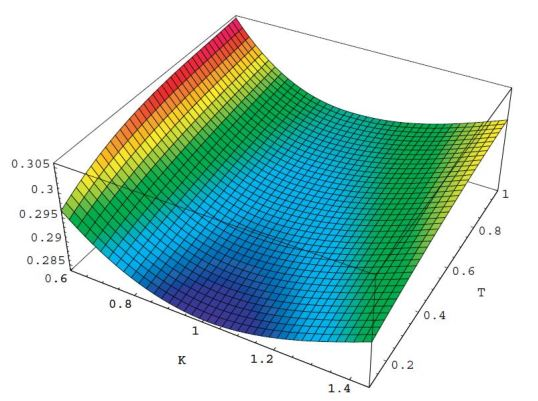
\includegraphics[width=0.70\textwidth]{fig1.JPG}
	\label{image1}
	\caption{Implied call volatilities as function of strike $K$ and time $t$.}
\end{figure}

\subsection*{Remarks}
\begin{enumerate}
\item[1.] Implied volatilities were calculated for the numerical results shown here by using both domestic and foreign zero coupon bonds to infer the discount factor used in the Black–Scholes formula for exchange rate call and put options. This ensures that the implied volatilities calculated for call and put options with the same strike price and maturity date are identical.

% For the numerical results shown here, implied volatilities were calculated
% by using both the domestic and foreign zero coupon bonds to infer the
% discount factor used in the Black–Scholes formula for exchange rate call
% and put options. This ensures that the implied volatilities calculated for call and put options with the same strike and maturity date are the same.
\item[2.] Inspection of Fig. 1 shows that for the default parameters used the at-the- money implied volatilities increase gradually as the maturity date
increases. The implied volatility smile curvature, evident in Figure \ref{image3}, is due to
the scaling process $\gamma$. This type of shape for the term structure of implied volatilities is  typical for observed currency options.
\end{enumerate}
 %%%%%%%%%%%%%%%%%%%%%%%%%%%%%%%%%%there is an image hereeeee
\newpage 
\begin{figure}[hp]
	\centering
		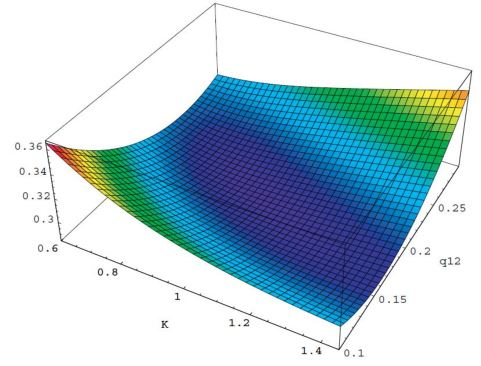
\includegraphics[width=0.70\textwidth]{fig2.JPG}
	\label{image2}
	\caption{Implied call volatility as a function of strike $K$ and scaling level $q^{1,2}$ with $q^{0,1}+q^{1,2} = 0.4.$}
\end{figure}
\subsection*{Remark}
\noindent
\par For a fixed maturity date $T$ = 0.25, Figure \ref{image4} shows implied volatilities for European call options as a function of the scaling level $q^{1,2}$. Here the normalization condition $q^{0,1}+q^{1,2} = 0.4$ is imposed to ensure that the at-the-money implied volatilities are approximately the same for different values of $q^{1,2}$. Note that by changing the magnitude of $q^{1,2}$ relative to $q^{0,1}$ the implied volatility curve can be changed from a predominately negatively skewed smile to a predominantly positively skewed smile.

This is generally only obtained for a variety of stochastic volatility models by using different values for the degree of correlation between the driving Wiener processes for the models. It is obtained more naturally and directly here by employing the %scaling levels $q0,1$ and $q1,2$.
% For a range of stochastic volatility models this is generally only obtained by using different values for the degree of correlation between the driving Wiener processes for the models. Here it is obtained more naturally and directly by using the 
scaling levels $q^{0,1}$ and $q^{1,2}$.

%%%%%%%%%%%%%%%%%%%%%%%%%%%%%%%%%%%%%% there is an image hereeee
\begin{figure}[hp]
	\centering
		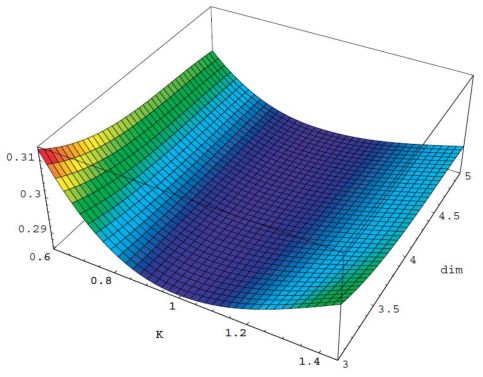
\includegraphics[width=0.70\textwidth]{fig3.JPG}
	\label{image3}
	\caption{Implied call volatility as a function of strike $K$ and dimension $v_2$ with $v_1 = v_2$}.
\end{figure}

\subsection*{Remark}
\noindent
\par For a fixed maturity date $T = 0.25$, Figure \ref{image3} displays implied volatilities as a
function of the strike $K$ and the dimension $v_2$ with $v_1 = v_2$. It can be seen that a
lower dimension produces more curvature for the implied volatility smile. For
higher dimensions some degree of curvature is still present. This is due to the
natural curvature produced by the random scaling process $\gamma$. 


%%%%%%%%%%%%%%%%%%%%%%%%%%%%%%%%%%%% there is an image hereeee
\newpage
\begin{figure}[hp]
	\centering
		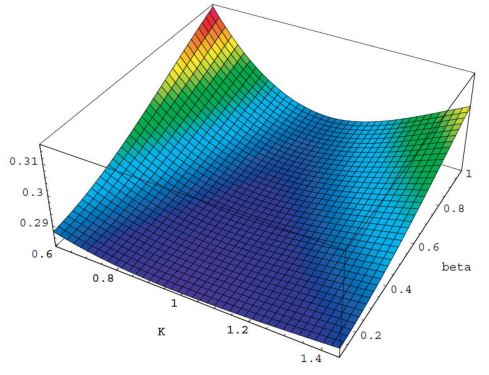
\includegraphics[width=0.70\textwidth]{fig4.JPG}
	\label{image4}
	\caption{Implied call volatility as a function of strike $K$ and scaling volatility $\beta$.}
\end{figure}

\subsection*{Remark}
\begin{enumerate}
\item[(1.)] Finally, Figure \ref{image4} shows implied volatilities as a function of the strike K and
scaling volatility $\beta$. Note the dramatic increase in curvature if the scaling
process $\gamma$ is made more volatile.
\item[(2.)] This figure shows the impact of using a random scaling process and its
effect on the curvature of implied volatilities.
\item[(3.)] The above figures illustrate how the curvature and skewness of the
implied volatilities of exchange rate options change depending on the
parameter choice for the MMM. From a practical point of view it is clear
that with realistic parameter choices one can capture using the above
parsimonious model the typical implied volatility surfaces of exchange
rate options.
\end{enumerate}

\chapter{CONCLUSION}
\noindent
\par %To describe the dynamics of a currency market, this project proposes a
% minimal market model with random scaling. The growth optimal portfolio and
% its various denominations in domestic and international currencies are
% represented using appropriate representations in this parsimonious and
% realistic model. Time transformed squared Bessel processes arise for each of
% the associated factors.\\
\par This project proposes a minimal market model with random scaling to describe the dynamics of a currency market. In this concise and realistic model, the growth optimal portfolio and its various denominations in domestic and international currencies are represented using appropriate representations. For each of the associated factors, time transformed squared Bessel processes emerge.\\
\par A random scaling process is also used to model the time transition. The particular time transformation was chosen to demonstrate the impact of random market activity. Because the model does not accept an equivalent risk-neutral martingale measure, European-style securities are priced using the fair pricing concept.
% \par Additionally, a random scaling process is used to model the time
% transition. The particular time transformation was chosen to illustrate the
% influence of market activity that is random. Because the model does not accept
% an equivalent risk neutral martingale measure, the fair pricing idea is used to
% price European style securities.\\

% \par Numerical results for the proposed three-factor model have been obtained, which show realistic implied volatility surfaces for European currency
% options. A powerful numerical expansion method is described that can be used to efficiently price European style derivatives.

\par The proposed three-factor model yielded numerical results that show realistic implied volatility surfaces for European currency options. A powerful numerical expansion method that can be used to efficiently price European-style derivatives is described.




%\begin{equation}\label{}
%
%\end{equation}
%
%\begin{equation}\label{}
%
%\end{equation}
%
%\begin{equation}\label{}
%
%\end{equation}
%
%\begin{equation}\label{}
%
%\end{equation}
%
%\begin{equation}\label{}
%
%\end{equation}
%
%\begin{equation}\label{}
%
%\end{equation}
%
%\begin{equation}\label{}
%
%\end{equation}
%
%\begin{equation}\label{}
%
%\end{equation}
%
%\begin{equation}\label{}
%
%\end{equation}
%
%\begin{equation}\label{}
%
%\end{equation}
%
%\begin{equation}\label{}
%
%\end{equation}
%
%\begin{equation}\label{}
%
%\end{equation}
%
%\begin{equation}\label{}
%
%\end{equation}
%
%\begin{equation}\label{}
%
%\end{equation}










\bibliography{Ali799}
\nocite{*}
\bibliographystyle{apacite}
\end{document}